% !TEX root = main.tex

\section{System design}
\subsection{Visual Filtering}

The simulations shown on Figs.~\ref{fig:glaucoma-filters} and \ref{fig:myopia-filters} were implemented using the Visual Impairments Simulator Chrome extension \cite{visual_impairments_simulator}. Simulating visual impairments through perceptual filters allows us to have an approximation to the experiences of users with vision loss conditions. Still, these tools are inherently limited; since visual disabilities are highly individualized, and no filter can perfectly replicate the subjective visual experience of~every~user.

\begin{figure}
    \centering
    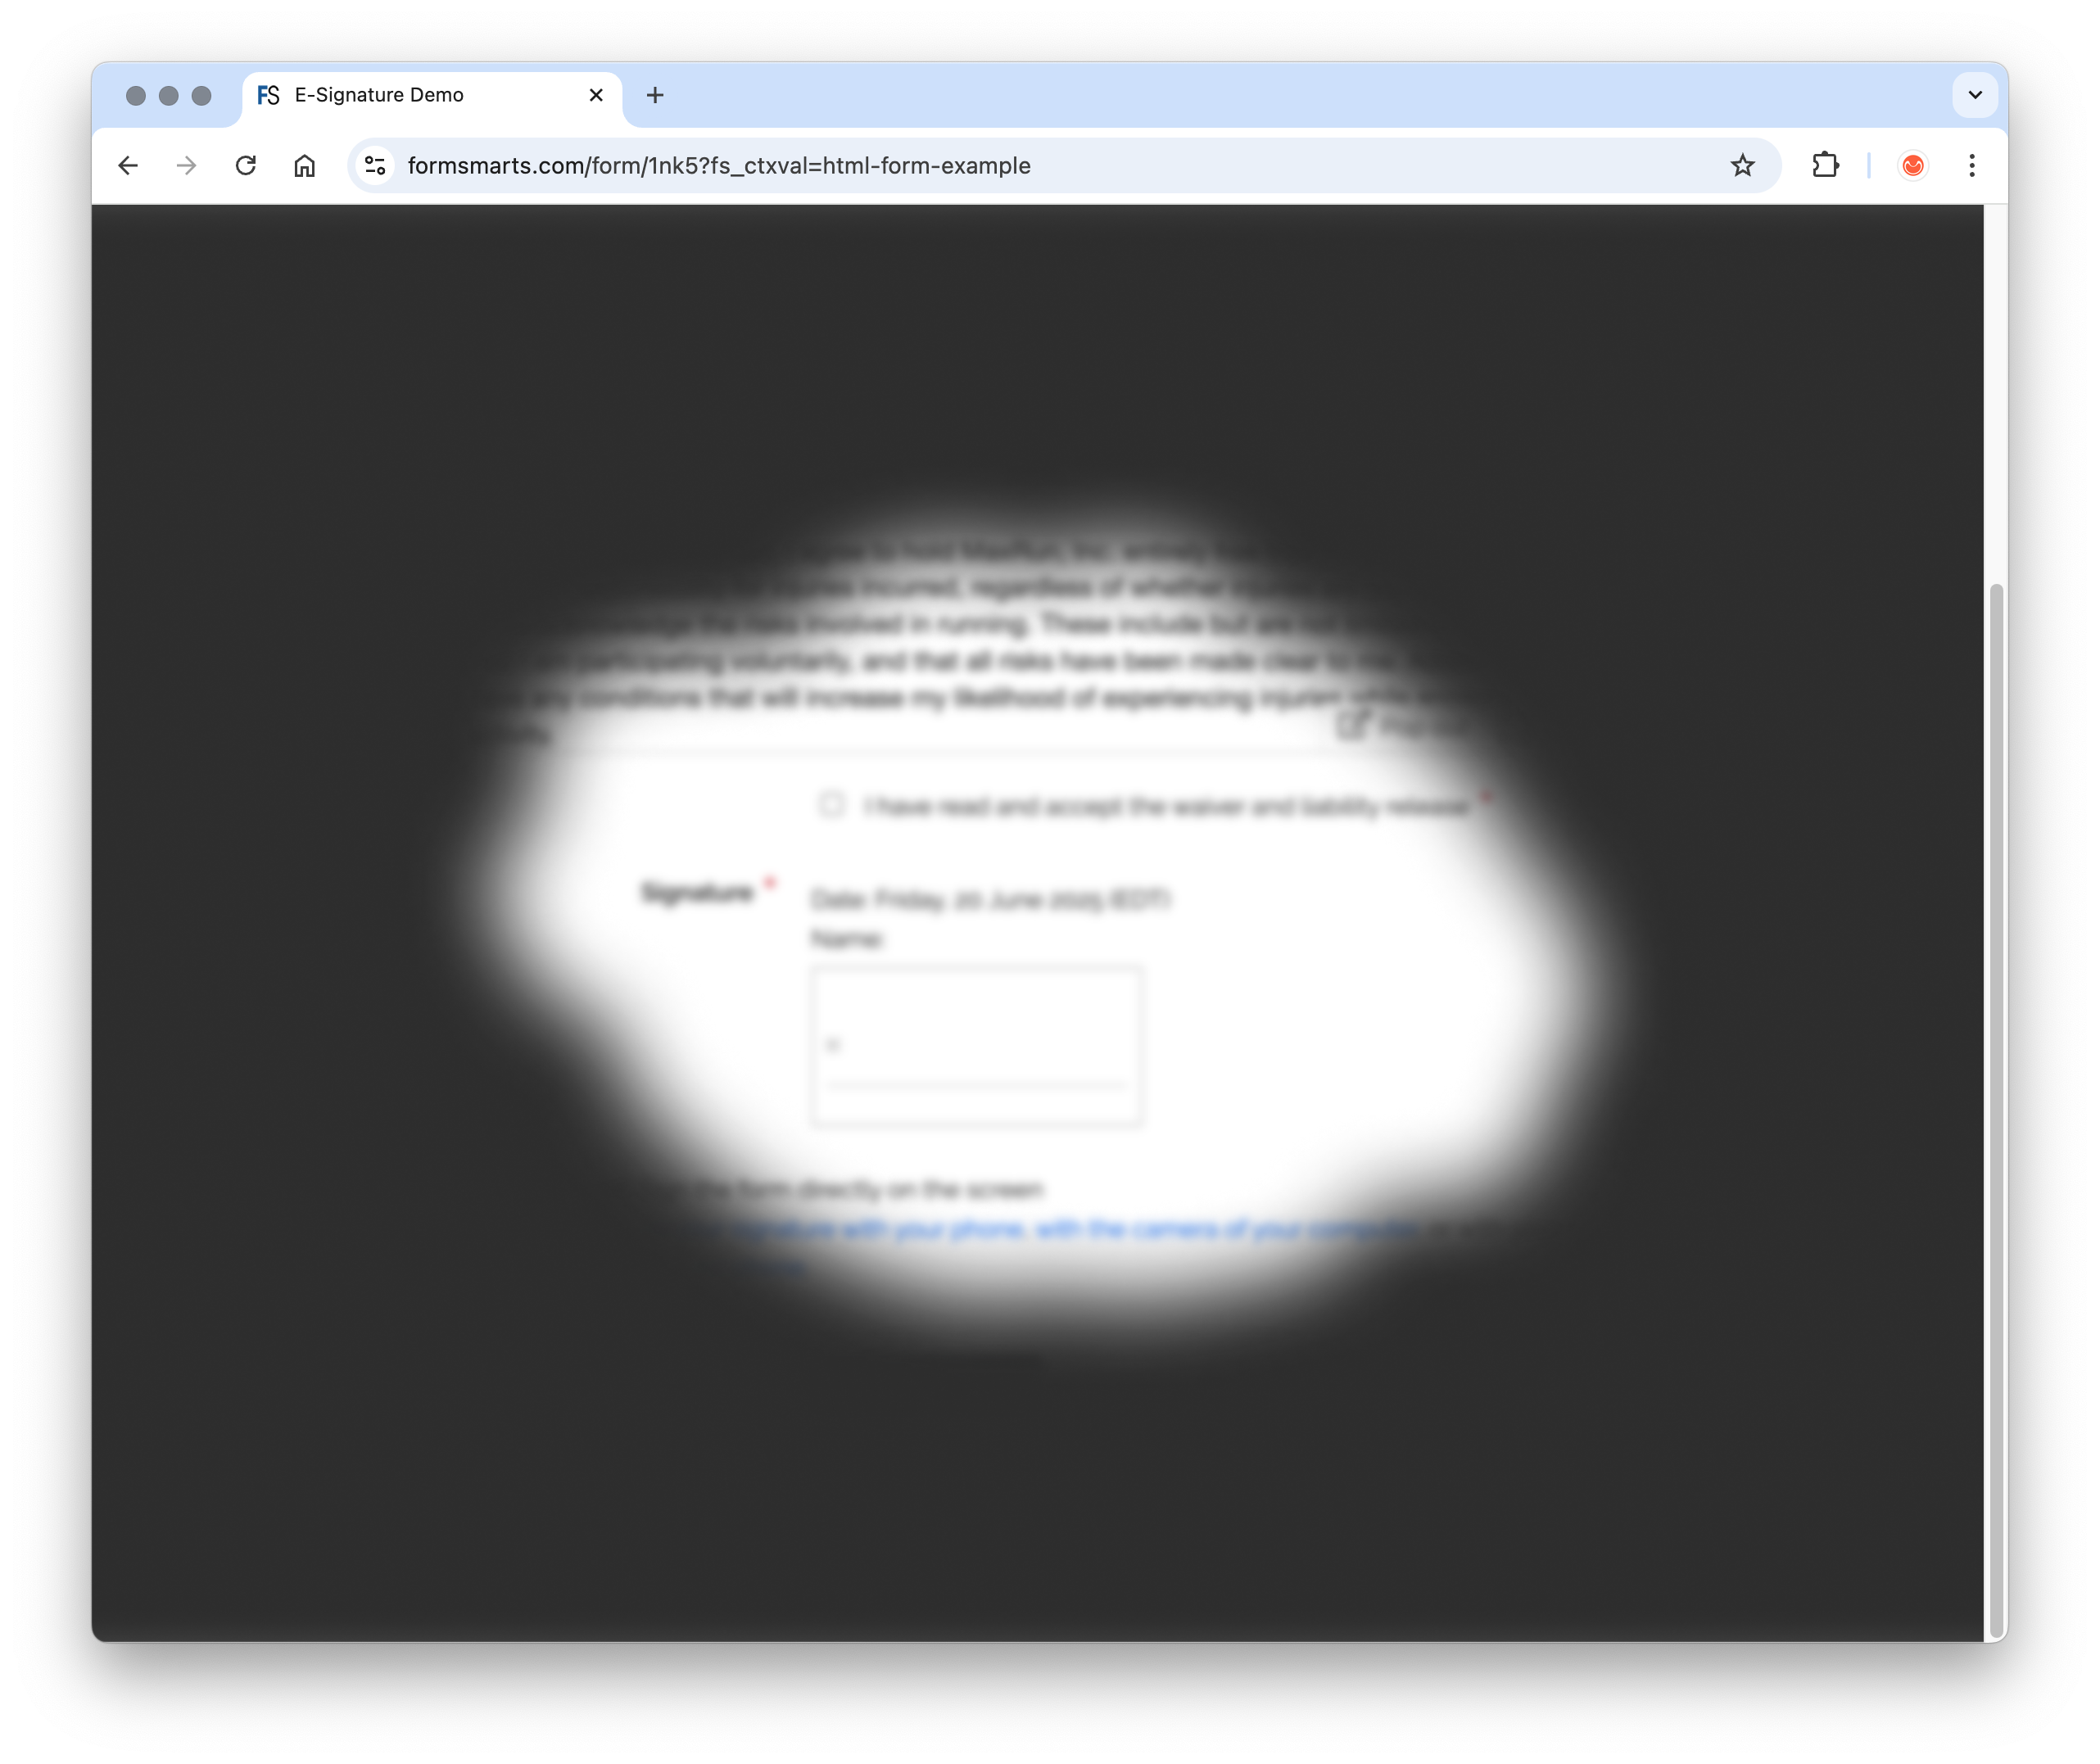
\includegraphics[width=115pt]{imgs/glaucoma-filter.png}
    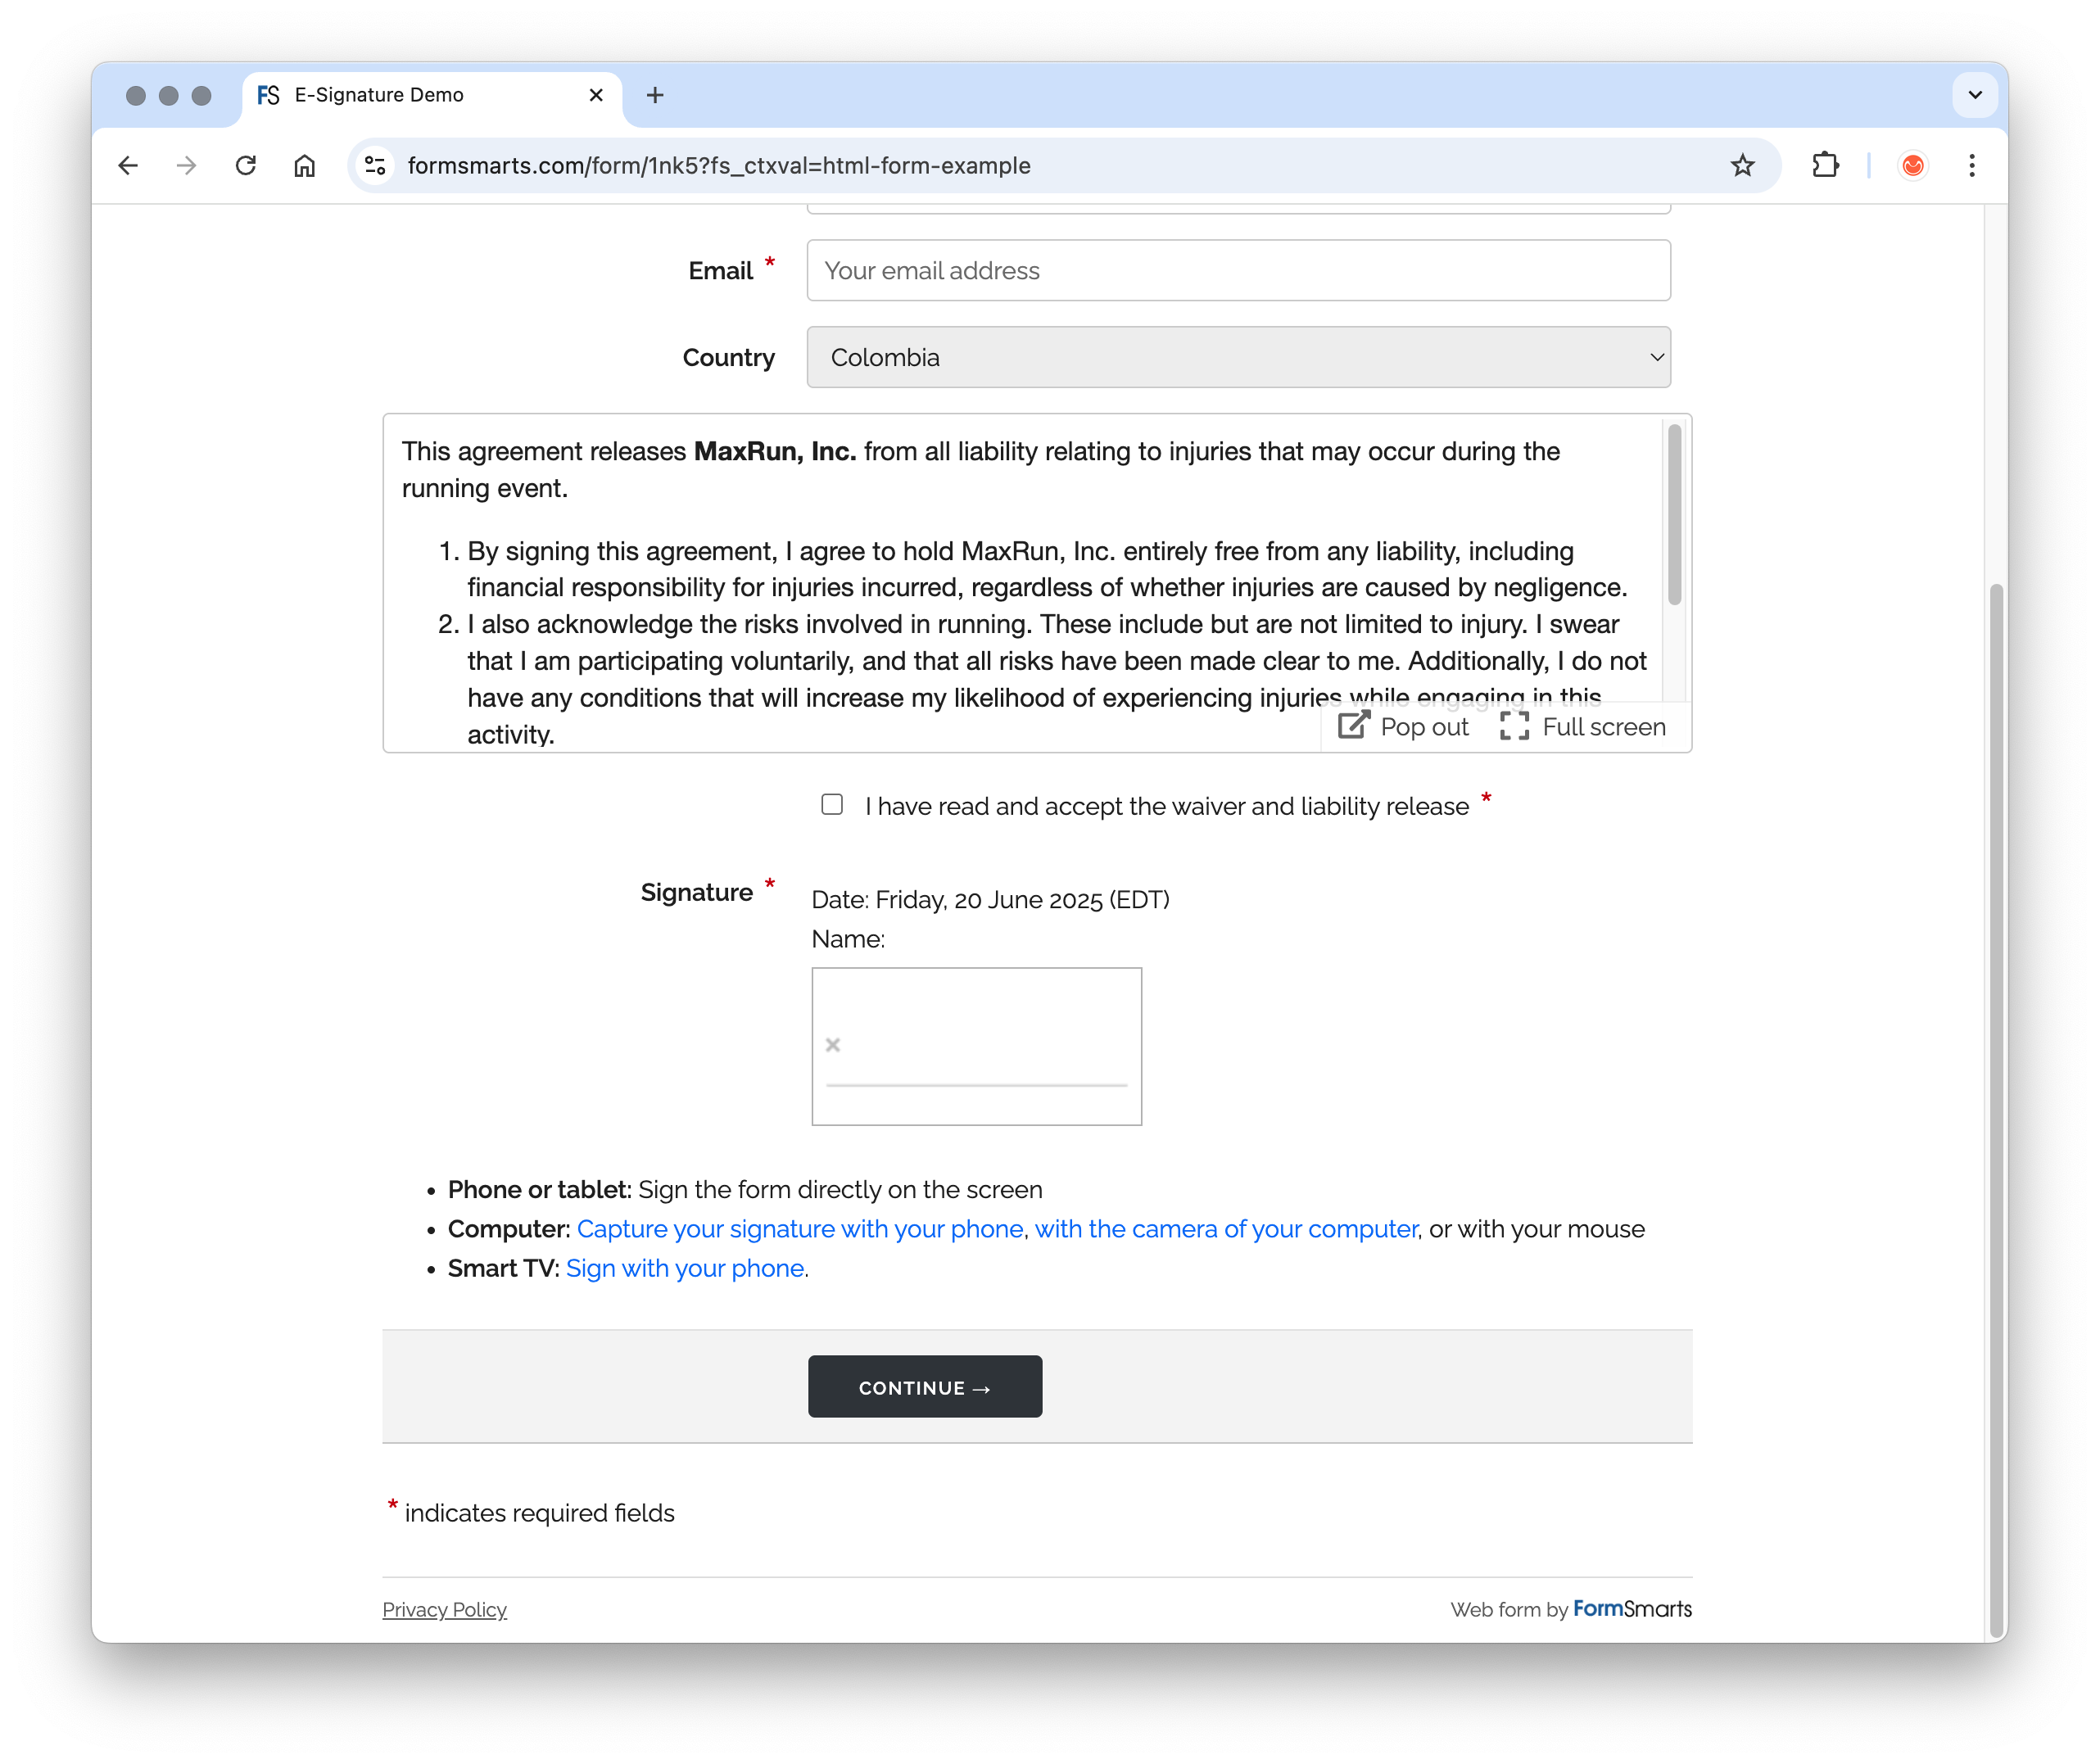
\includegraphics[width=115pt]{imgs/no-glaucoma-filter.png}
    \caption{Left: Glaucoma filter applied to an example form requiring a signature. The "Submit" button is no longer visible, making it difficult to locate. Right: Original version.}
    \vspace{-13pt}
    \label{fig:glaucoma-filters}
\end{figure}

\begin{figure}
    \centering
    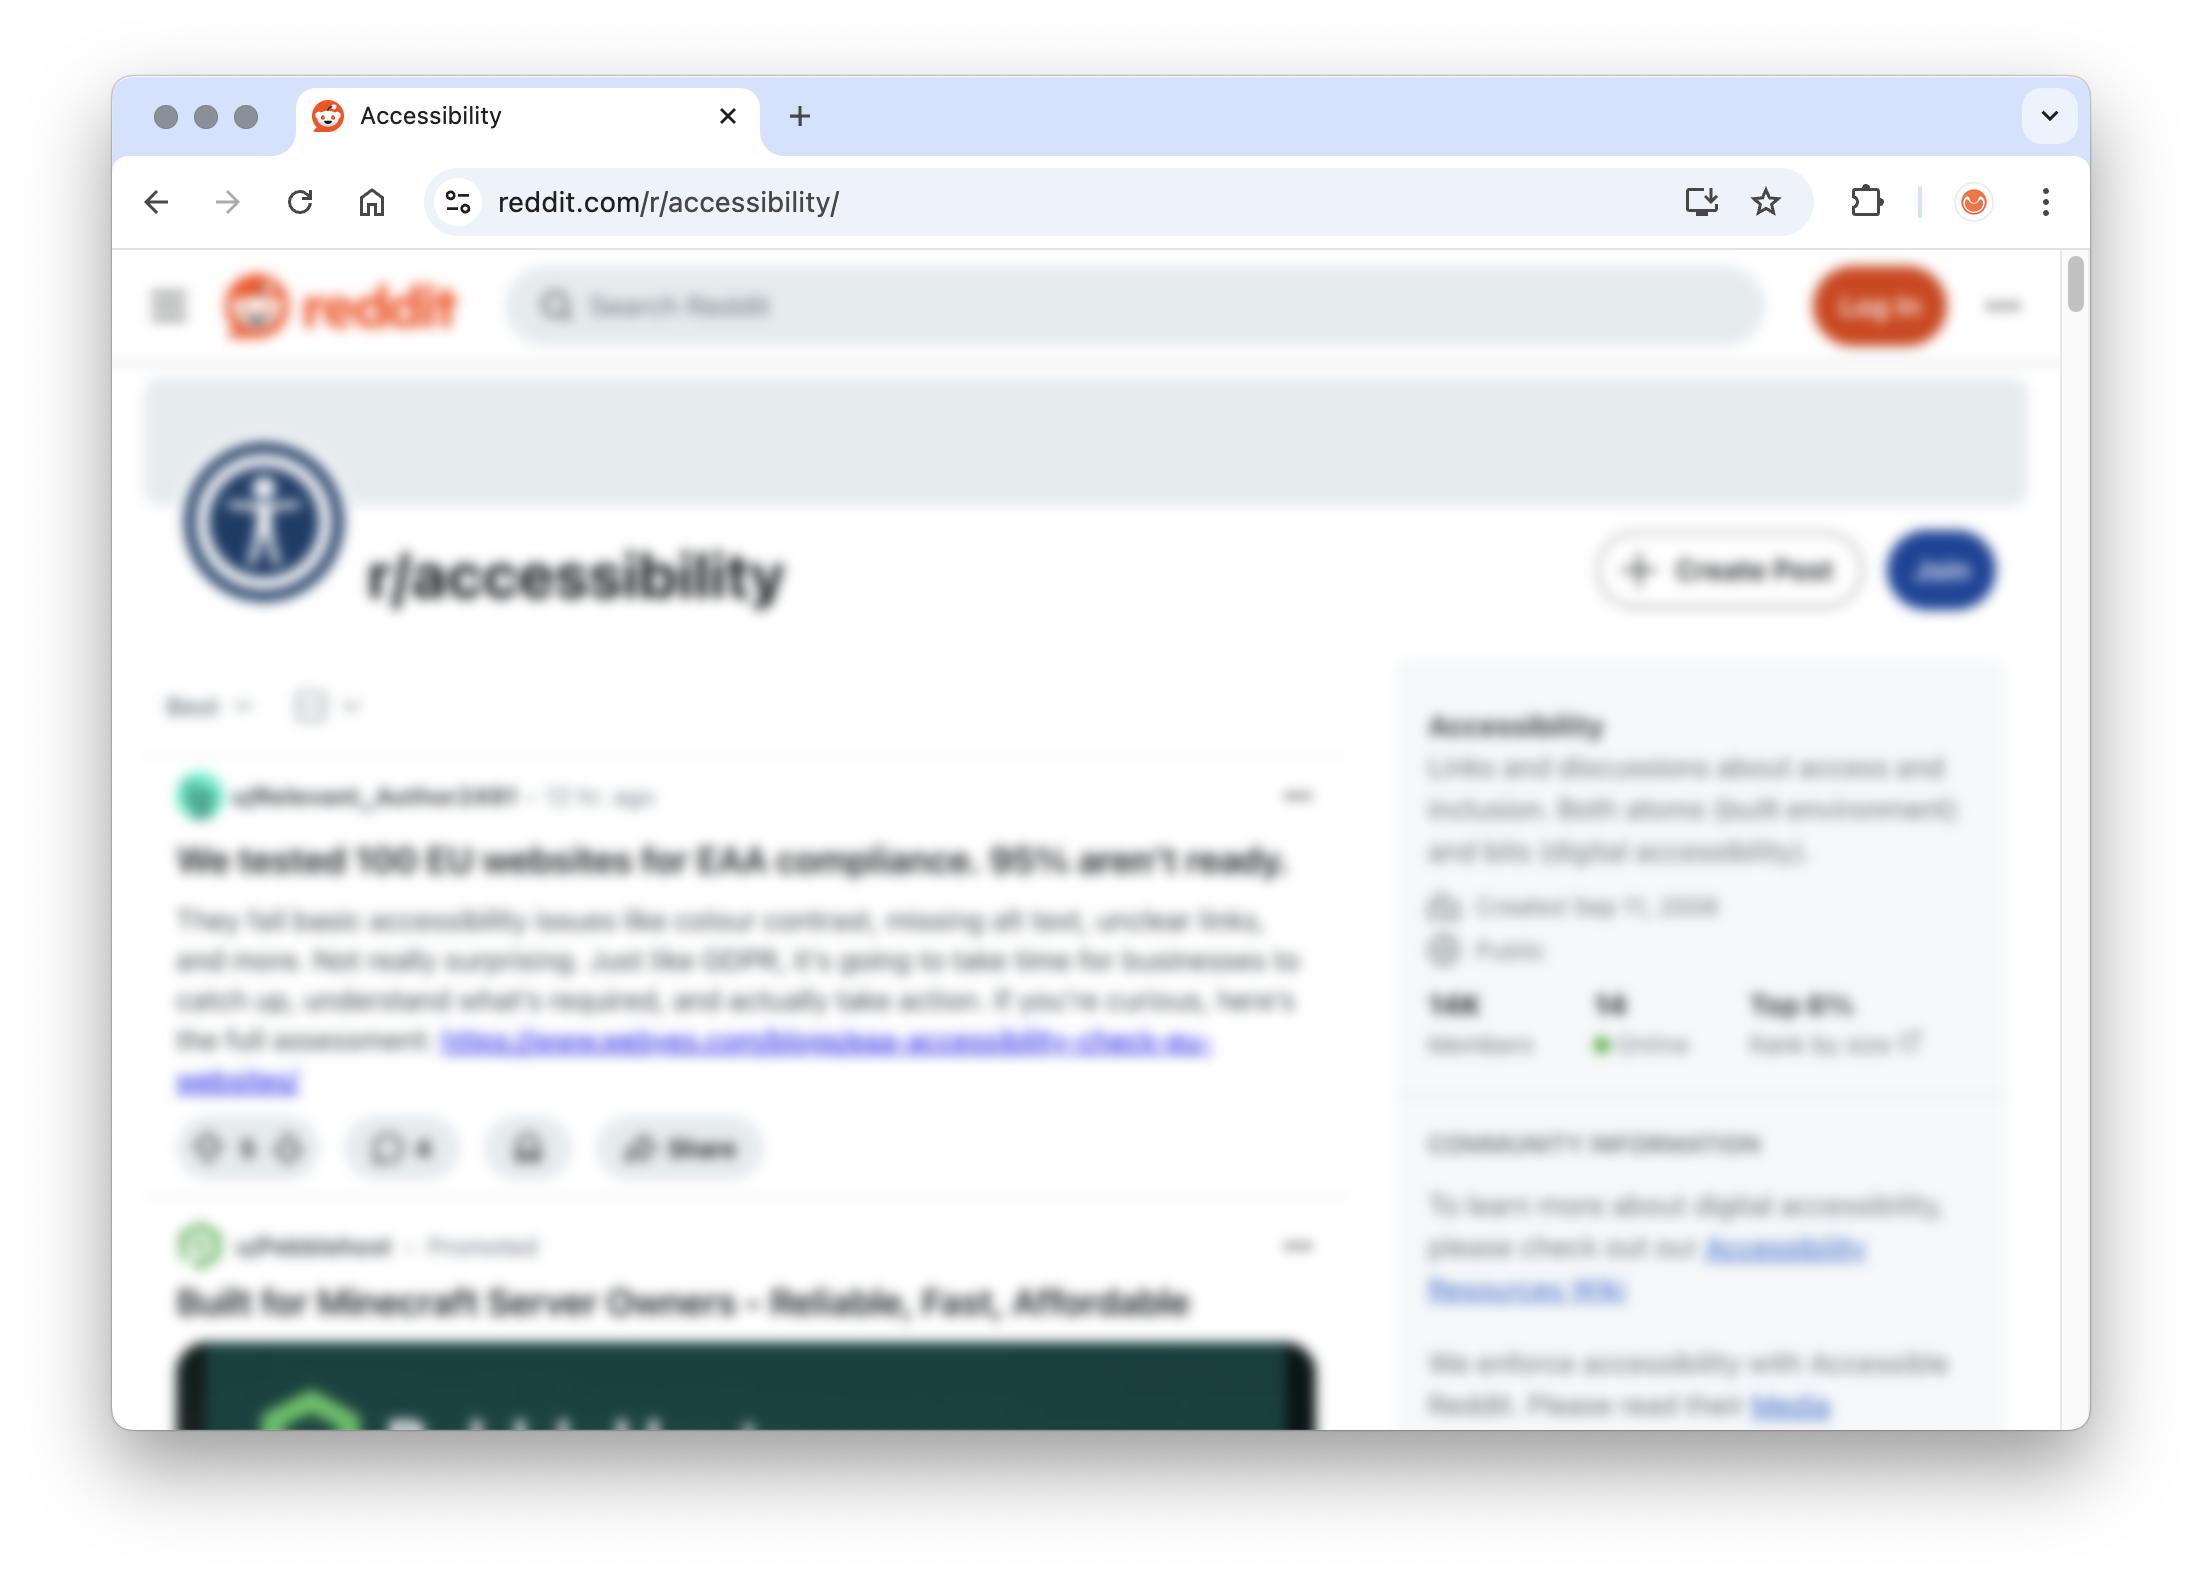
\includegraphics[width=115pt]{imgs/myopia-filter.png}
    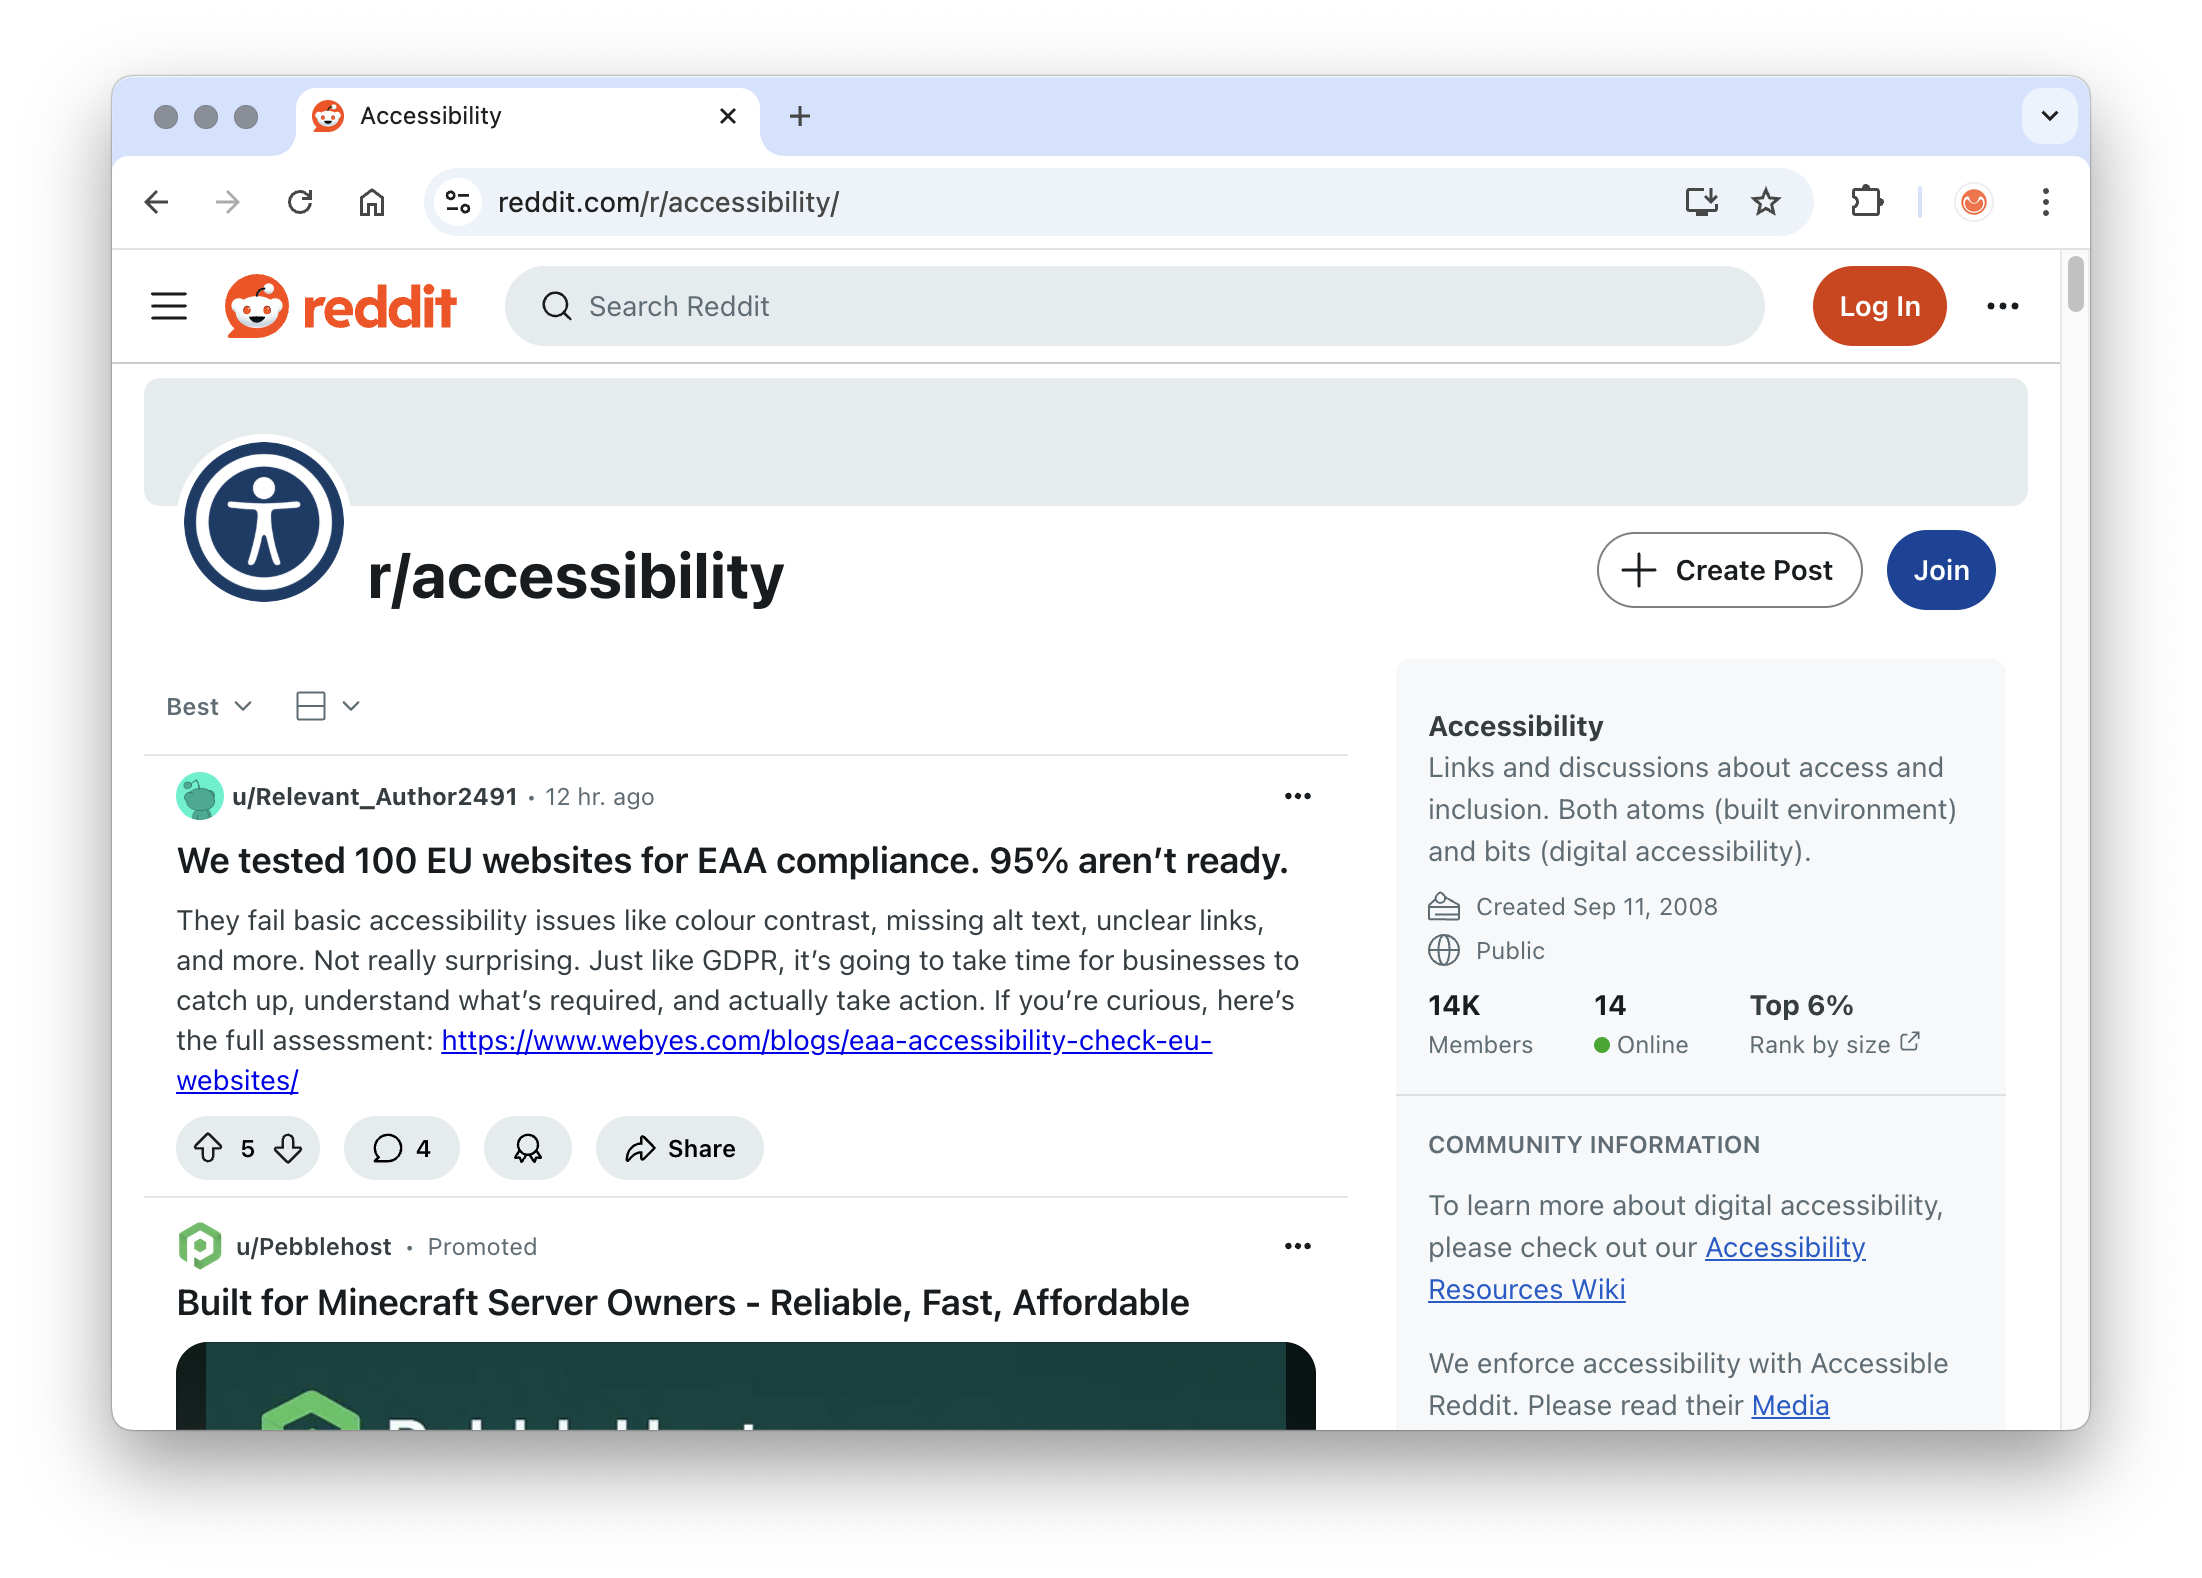
\includegraphics[width=115pt]{imgs/no-myopia-filter.png}
    \caption{Left: Myopia filter (-3 diopters) applied to a social media webpage, reducing clarity and edge sharpness. Right: Original version.}
    \vspace{-13pt}
    \label{fig:myopia-filters}
\end{figure}

% * The paper lacks an analysis of the target population and the specific visual impairments considered. The authors do not clearly articulate which types of visual impairments are modeled, their characteristics, or whether the chosen visual filtering techniques can adequately represent their impact on Web browsing.

In light of these considerations, the beta testing of this agent will focus on a defined set of visual impairments. The prototype includes simulations of glaucoma (peripheral field loss and tunnel vision\cite{Cassel2021EyeBook}), diabetic retinopathy (scattered blind spots and patchy visual fields\cite{Cassel2021EyeBook}), cataracts (global blurriness and reduced contrast sensitivity\cite{Cassel2021EyeBook}), and myopia (blur at distance with varying levels of diopter correction\cite{Cassel2021EyeBook}). These conditions were selected as representative examples because they encompass distinct perceptual characteristics, in ways that reflect known physiological effects.

In addition, experimenting with different viewports, font sizes, and other browser configurations\cite{chiou2024automatically} will be done to test how these factors affect usability.

Future work involves collaboration with ophthalmologists and vision science experts to improve the clinical accuracy of these filters. Their insight can guide the calibration of filter parameters and help us design simulations that more closely resemble the lived experiences of users.

\subsection{Assistive output integration}

\begin{figure}
    \centering
    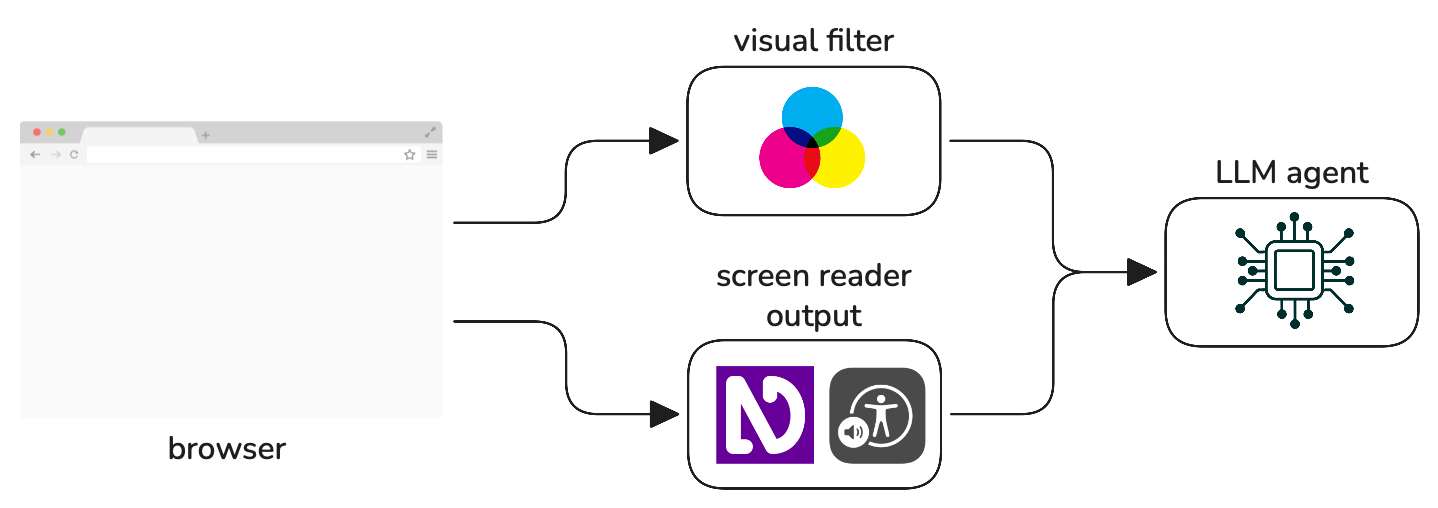
\includegraphics[width=1\linewidth]{imgs/flow.png}
    \caption{Proposed pipeline for the agent feeding inputs}
    \vspace{-13pt}
\label{fig:pipeline}
\end{figure}

The agent must capture what an assistive technology user would hear and do. For screen reader output, we can integrate a driver API, such as Guidepup\cite{guidepup2025} that programmatically controls VoiceOver\cite{voiceover2024} or NVDA\cite{nvda2024}.
This driver issues the same keyboard commands a user would and exposes the spoken utterances\cite{guidepup2025}. The agent framework would invoke this API at each step and record the resulting string of text (including element role, name, state) as sensory input.

% * Explain how issues are detected from agent logs — show concrete log features, detection rules/heuristics or classifiers, and example mappings (log → issue).

For navigation logs, the agent can log focus events. As the agent presses Tab, arrow keys, click, enter, etc., we can attach listeners to record each focus transition and action. This yields a sequence of elements visited in order, that can then be executed using a browser automation framework, namely Playwright\cite{playwright2025}, Selenium\cite{garcia2024selenium}, or Kraken\cite{ravelo2023kraken}.

% * metadata, model-based representation of what the user does. click and all interactions also is enriched by ARIA labels

The agent can also log accessibility metadata, thereby having the ability to cross-check perception. This means reading the ARIA attributes for the current focused element. For instance, when an element is in focus, the agent can query its ARIA label, via the \ac{AOM} or other APIs. This is then compared to the other information (visual, audio). If the visible text of a button says “Search” but its ARIA label is “Submit” that mismatch is noteworthy. Altogether, ARIA attributes and accessibility metadata enrich the logs by providing a semantic model of user actions and interface states, allowing for more precise analysis and how accessibility features are utilized or bypassed. This is useful for verifying consistency, which is one of the guidelines on \ac{WCAG} and IBM's\cite{ibm2025accessibility}. 

In general, the resulting logs constitute a detailed record of the agent's navigation path, enabling systematic analysis of interaction patterns. They can be examined to identify instances where interface elements were bypassed, or to detect deviations from the expected focus order. Furthermore, replaying recorded sessions facilitates a nuanced assessment of element discoverability, the interpretation of screen reader output, and the factors influencing task completion or failure. Together, these multimodal data streams comprehensively characterize the agent's perceptual state at each interaction step. 


\subsection{Decision and Action Module}


Our approach consists of prompting the agent with a basic user goal. E.g. “given this screenshot and screen reader transcript, where is the 'Submit' button?”. The agent will then attempt to complete the task, using the screen reader and seeing through the visual impairment filter applied to the~interface.
Consider one scenario which may involve an \ac{AI} agent attempting to find and click a "Submit" button after filling out a form. With a glaucoma filter applied (see Fig.~\ref{fig:glaucoma-filters}), the button may become difficult to distinguish due to peripheral blur or low contrast. The agent has to decide which interaction method works best (pointer, keyboard, etc) and execute the decision.

\subsection{Workflow Definition}

Each testing task needs to be defined in advance. This can be done either with a script or using natural language to define a goal. Then, the agent will execute said task in a closed loop that has a completion or failure condition. All in all, the loop can be structured in this way (see Fig.~\ref{fig:pipeline}).

\underline{Steps:} Perception (capture current state: screenshot, screen-reader output, optionally \ac{AOM} information) $\rightarrow$ Decision (agent chooses next action, e.g., LLM generates plan and writes a rule-based script that framework follows) $\rightarrow$ Action (execute step) $\rightarrow$ Measure (log outputs, check goal, repeat).


\subsection{Metrics and Analysis}

After execution is complete, some of the metrics we propose that the system displays are both classic usability and accessibility-specific. These include the agent's task success rate, efficiency (measured by completion time or number of actions), and the frequency of interaction errors, missed clicks or incorrect actions that require backtracking. 

We also include the consistency between screen reader output and the visible \ac{UI}, flagging any mismatches between spoken labels and on-screen text or roles. Visual robustness can also be examined by analyzing the webpage before the filter, discovering layout faults like overlapping or off-screen elements, among others. 

Heuristic checks are performed during testing, among them are verifying that text scales appropriately in high-contrast or large-text modes and monitoring for navigation loops. Throughout the process, we aggregate logs of the agent's actions and screen reader output for offline analysis, enabling manual review or further explanation by the agent. By comparing these metrics across different simulated conditions, we can quantify the impact of visual impairments on usability and identify both layout and semantic accessibility issues.


\section{Evaluation}

To investigate the feasibility and effectiveness of using autonomous AI agents for accessibility evaluation, we pose several research questions. We ask whether autonomous AI agents can realistically emulate the interaction patterns of users with vision-related impairments when navigating web interfaces. This includes examining which visual filters or perceptual constraints most effectively represent different types of visual impairments in a simulated context, and what design principles are necessary for agents to approximate visual impairments through perception-based (rather than code-aware) interaction.

We also explore whether these agents can surface accessibility problems that static tools overlook, like poor contrast visibility, confusing focus order, or dynamic content that is not screen-reader friendly, to name a few. Another important question is whether agent-based testing, when combined with simulated impairments, can produce accessibility assessments that are reliable and generalizable. We are interested in the extent to which these systems can internalize accessibility heuristics through observation of human interaction data, rather than relying solely on static rule sets.

Finally, we investigate how combining simulated visual impairment filters with screen reader output affects the agent's ability to detect accessibility issues, and whether multi-modal input can uncover problems, say, missing alt text, that would not surface if using only visual filtering.

To evaluate our approach, we will conduct experiments on a curated set of benchmark web pages, including public sites with documented accessibility issues. Inspired by Alameer et al.\cite{alameer2016detecting}, who compiled websites with internationalization challenges, we may extend our benchmarks to include similar cases. For each page, we will define representative tasks, and assess agent performance across different visual filters and input modalities. We plan to complement these quantitative results with qualitative feedback from accessibility experts and targeted user studies, to further validate the effectiveness and generalizability of agent-based accessibility testing.

\vspace{-4pt}